\documentclass[11pt, oneside]{article}   	% use "amsart" instead of "article" for AMSLaTeX format
\usepackage{geometry}                		% See geometry.pdf to learn the layout options. There are lots.
\geometry{letterpaper}                   		% ... or a4paper or a5paper or ... 
%\geometry{landscape}                		% Activate for rotated page geometry
%\usepackage[parfill]{parskip}    		% Activate to begin paragraphs with an empty line rather than an indent
\usepackage{graphicx}				% Use pdf, png, jpg, or eps§ with pdflatex; use eps in DVI mode
								% TeX will automatically convert eps --> pdf in pdflatex	
\graphicspath{ {white-paper-figures/} }	
\usepackage{amssymb}
\usepackage{amsmath}
\usepackage{siunitx}
\sisetup{group-separator = {,}}

%SetFonts

%SetFonts


\title{Optimal Inventory Allocation for E-commerce Fulfillment}
\author{Christopher Holloman \\ Chief Data Scientist \\ Advanced Analytics Practice \\ Information Control Company}
\date{Last updated: \today}							% Activate to display a given date or no date

\begin{document}
\maketitle

Given the growth of e-commerce, it is increasingly important for retailers to optimally allocate inventory to fulfillment centers to ensure that goods can be delivered to customers' home addresses quickly. Optimal allocation must account for two primary factors:

\begin{itemize}
\item Cost of delivering units from fulfillment centers to delivery addresses
\item Length of time required to fulfill orders to delivery addresses from fulfillment centers
\end{itemize}

In addition to these two primary factors, there are a host of other factors that could be considered in solving the allocation problem.  Key among those are the cost of transferring units between fulfillment centers to respond to shifts in demand and decisions about whether to fulfill on-line orders from stores instead of dedicated fulfillment centers.  In proposing a solution to the optimal allocation problem, we assume that no transfers are made between fulfillment centers and that e-commerce orders are fulfilled only from dedicated fulfillment centers (\emph{i.e.}, no fulfillment from stores).

\section{Assumptions}

There are many problems to be solved in optimizing sales of an individual SKU.  We will not address all of those problems here but will assume that the retailer has solutions and procedures in place for several problems:

\begin{itemize}
\item How to forecast the number of units sold in different geographic regions (\emph{e.g.}, zip codes, markets, regions, etc.)
\item How to quantify the uncertainty about the number of units to be sold in each region
\item How to determine which e-commerce fulfillment center fulfills each on-line order
\end{itemize}

For the purpose of this paper, we assume that the retailer has solved the first two problems by developing a statistical model forecasting the number of units that will be purchased through the online channel in each of several regions.  We also assume the retailer has quantified their uncertainty in those forecasts.  Further, we assume that the retailer has a set of rules specifying the logic for selecting which fulfillment center will fulfill each order.

\section{Forecasting Online Sales}

When forecasting on-line sales, we start with a set of households, denoted $\mathcal{H}$.  Although it is possible to forecast purchases at the household level, forecasting models are usually build at an aggregate level.  For example, we might create forecasts within political boundaries (\emph{e.g.,} county or state) or within designated marketing areas.  Define a partition $\mathcal{P}$ of $\mathcal{H}$, so $\mathcal{P} = \{P_1, P_2, ..., P_K \}$, where $P_k \cap P_{k'} = \emptyset$ for all $k$ and $k'$ and $\bigcup_k P_k = \mathcal{H}$.  The elements of this partition constitute the set of regions for which forecasts are created.

For simplicity of modeling, we assume that forecasting for the SKU of interest has been performed taking a Bayesian approach, so the retailer has posterior distributions for each of the parameters in the forecasting model.  Denote the historical demand data from which the forecasting model was constructed $\mathbf{Y}$ and the historical independent variables used to predict demand $\mathbf{X}$.  Denote the set of parameters in the model $\boldsymbol{\theta}$.  Using a Bayesian approach, the forecasting model has a posterior distribution for $\boldsymbol{\theta}$,

$$\pi (\boldsymbol{\theta} \mid \mathbf{Y}, \mathbf{X}) \propto \pi (\mathbf{Y} \mid \boldsymbol{\theta}, \mathbf{X}) \pi (\boldsymbol{\theta}).$$

\noindent For the purpose of forecasting future sales, we assume that future values of the independent variables are known.  We denote those future values $\mathbf{X}^*$.  Similarly, we denote future values of demand $\mathbf{Y}^*$.  The predictive distribution of $\mathbf{Y}^*$ is

$$\pi (\mathbf{Y}^* \mid \mathbf{X}^*, \mathbf{Y}, \mathbf{X}) = \int_{\boldsymbol{\Theta}} \pi (\mathbf{Y}^* \mid \boldsymbol{\theta}, \mathbf{X}^*) \pi (\boldsymbol{\theta} \mid \mathbf{Y}, \mathbf{X}) d \boldsymbol{\theta}$$.

\noindent We assume that forecasting is performed over a finite set of time points, $1, \ldots, T$ within each region.  The forecast in region $k$ at time $t$ is denoted $Y_{kt}^*$.  The total demand across all time points and regions is denoted $D^*$, and

$$D^* = \sum_{t = 1}^T \sum_{k = 1}^K Y_{kt}^*.$$

In this formulation, $D^*$ can be interpreted as the total number of units the retailer will sell over a pre-specified time period.  Beyond the planned time period, it is usually expected that the price will be marked down to accelerate the rate of sales for remaining inventory.

\section{Determining the Buy}

For our determination of optimal allocation, we assume that the number of units purchased has already been determined.  Denote the total number of units purchased $b$.  Typically, the actual buy is selected to ensure a low probability that demand exceeds supply.  For example, we might select the $95^{th}$ percentile of the predictive distribution of $D^*$, giving a $5\%$ probability that demand will exceed supply.

\section{Fulfillment Centers}

Denote the set of fulfillment centers for e-commerce orders $\mathcal{F}$.  We use $J$ to denote the total number of fulfillment centers in $\mathcal{F}$.

\section{Cost function}

There are two primary factors associated with optimal allocation

\begin{itemize}
\item Cost of delivering units from fulfillment centers to delivery addresses
\item Length of time required to fulfill orders to delivery addresses from fulfillment centers
\end{itemize}

Both of these factors tend to increase as distance between the fulfillment center and the household increases.

The total cost associated with these two factors can be written as a function.  Denote this cost function $c \colon \mathcal{F} \times \mathcal{H} \mapsto \mathbb{R}^+$.  This function may be complicated, but it is typically a straightforward linear equation with fixed and variable cost components.  Denote the distance (\emph{e.g.}, in travel miles) between two points $d_1(\cdot, \cdot)$.  Denote a second distance metric that describes delivery time between fulfillment center and household $d_2(\cdot, \cdot)$  This second distance metric is intended to capture cost like lost future sales due to slow delivery.  The cost function can then be described as

$$c (f, h) = \gamma_{1} + \gamma_{2} d_1(f, h) + \gamma_{3} d_2(f, h),$$

\noindent where $\gamma_{1}$, $\gamma_{2}$, and $\gamma_{3}$ are positive values representing fixed cost, variable cost associated with distance travelled, and variable cost associated with time to deliver the product to the household, respectively.

\section{Fulfillment Rules}

Each business is unique in determining the rules it follows for fulfillment.  Fulfillment rules specify how each household placing an order will be assigned to the fulfillment center that will fulfill the order.  We assume that these rules have been specified by the business and are not being optimized as part of the allocation optimization problem.

\section{Accelerating Sales Rate}

Retailers use markdowns to accelerate the rate of sales of inventory that remains after a pre-specified amount of time has passed.  Denote the true demand during the pre-specified time period $d^*$.  When $d^* < b$, there are $b - d^*$ excess units to be sold.  These units are typically sold at a price resulting in a lower AUR than during the planned sales period.  We assume that the AUR for excess units can be expressed using a function $m \colon \mathbb{I}^2 \mapsto \mathbb{R}^+$.  A typical function describing this relationship would be

$$m (b, d^*) = r \exp \{- \delta (b - d^*) \},$$

\noindent where $r$ is the AUR during the planned sales period and $\delta$ is a parameter controlling how much markdown is required to sell excess inventory.

\section{Initial Allocation and Value}

For each of the $J$ fulfillment centers, our goal is to specify the number of units to be initially placed in each fulfillment center.  Let $\alpha_{jt}$ denote the inventory in fulfillment center $j$ at time $t$.  The initial allocation to fulfillment center $j$ is denoted $\alpha_{j0}$.

Given an initial allocation, a set of fulfillment rules, a cost function, an AUR value, a formula for AUR for units sold after the planned sales period, and a set of known demand values, it is possible to calculate a total value for an allocation rule as

\begin{align*}
\nu(\alpha_{10}, \alpha_{20}, \ldots, \alpha_{J0}, \mathbf{y}^*) = &br \mathrm{I}_{\{b \leq d^*\}} \\
&+ \left( d^*r + m(b, d^*) \} \right) \mathrm{I}_{ \{ b > d^* \} } \\
&+ \sum_{t = 1}^T \sum_{k = 1}^K \sum_{i = 1}^{n_{kt}} c (f_{tki}, h_{tki}),
\end{align*}

\noindent where $\mathrm{I}_{\{ \cdot \}}$ is the indicator function taking a value of $1$ if its subscript is true and $0$ otherwise, $n_{kt}$ is the number of households in region $k$ placing orders at time $t$, $h_{tki}$ is the $i^{th}$ household placing an order in region $k$ at time $t$, and $f_{tki}$ is the fulfillment center delivering to household $h_{tki}$.  The first line of the equation is the total sales value (number of units bought time AUR) when fewer units are purchased than the amount of demand during the planned sales period.  The second line is the total sales value when more units are purchased than the number for which there is demand at full price.  The third line is the cost of delivery.

While it is possible to calculate the value if future purchases are known, the future purchases are a random variable.  Consequently, instead of optimizing value, we optimize expected value, $\mathbb{E}[\nu]$.

$$\mathbb{E}[\nu \mid \alpha_{10}, \alpha_{20}, \ldots, \alpha_{J0}] = \int_{\mathbf{Y}^*} \nu(\alpha_{10}, \alpha_{20}, \ldots, \alpha_{J0}, \mathbf{Y}^*) \pi (\mathbf{Y}^* \mid \mathbf{X}^*, \mathbf{Y}, \mathbf{X}) d \mathbf{Y}^*$$.

\section{Implementation}

Calculation of $\mathbb{E}[\nu]$ for an initial allocation is intractable for even the simplest fulfillment rules.  Instead, we perform the optimization using a Monte Carlo approach.  The approach can be summarized as follows:

\begin{enumerate}
\item Generate a list of potential initial allocation values $\boldsymbol{\alpha}^{(1)}, \boldsymbol{\alpha}^{(2)}, \ldots, \boldsymbol{\alpha}^{(G)}$.
\item Loop through the sets of allocation values $g = 1, 2, \ldots, G$.
\begin{enumerate}
\item Loop through multiple iterations $l = 1, 2, \ldots, L$.
\begin{enumerate}
\item Generate a random draw of $\boldsymbol{\theta}$ from its posterior distribution.
\item Generate a random draw of $\mathbf{Y}^*$ from its posterior distribution, conditional on the drawn value of $\boldsymbol{\theta}$.
\item Loop through time points executing the fulfillment and transfer rules.
\item Record total value obtained.
\end{enumerate}
\item Average the $L$ calculated total values to obtain an estimate of expected total value.
\end{enumerate}
\item Select the initial allocation combination with the greatest expected total value.
\end{enumerate}

\section{Example}

\subsection{Problem Setup}

As a proof of concept, we implemented the recommended strategy on a simulated dataset.  A set of \SI{10000} households were generated and randomly assigned a location on the unit square.  Four fulfillment centers were also randomly assigned locations on the unit square.  The households were grouped into eight regions.  The locations of households, their assigned regions, and the locations of the fulfillment centers are shown in Figure~\ref{fi:hhfclocs}.

\begin{figure}
\centering
\includegraphics{hh-fc-locations}
\caption{Household locations (colored dots) by region with fulfillment center locations (numbers).}  \label{fi:hhfclocs}
\end{figure}

Within each of the eight regions, we specified a data distribution consisting of a Poisson distribution with a mean following an exponential decay curve.

$$Y_{kt}^* \mid \boldsymbol{\theta}_{k} \sim Poi(\mu_{kt})$$
$$\mu_{kt} = \theta_{1k} \exp \{ -t / \theta_{2k} \}.$$

\noindent We note that this model is somewhat simplistic since observations are conditionally independent, a scenario which is unlikely in a real forecasting situation.

Rather than generate values of $\mathbf{Y}$ and derive posterior distributions for the $\boldsymbol{\theta}$ parameters, we directly specified a hypothetical posterior distribution for each parameter.  The $95\%$ credible intervals for the cumulative demand curve derived from those posterior distributions in each region is shown in Figure~\ref{fi:demcurve}.  For this example, we set $T = 100$, so the demand curve is shown for $t = 1, 2, \ldots, 100$.

\begin{figure}
\centering
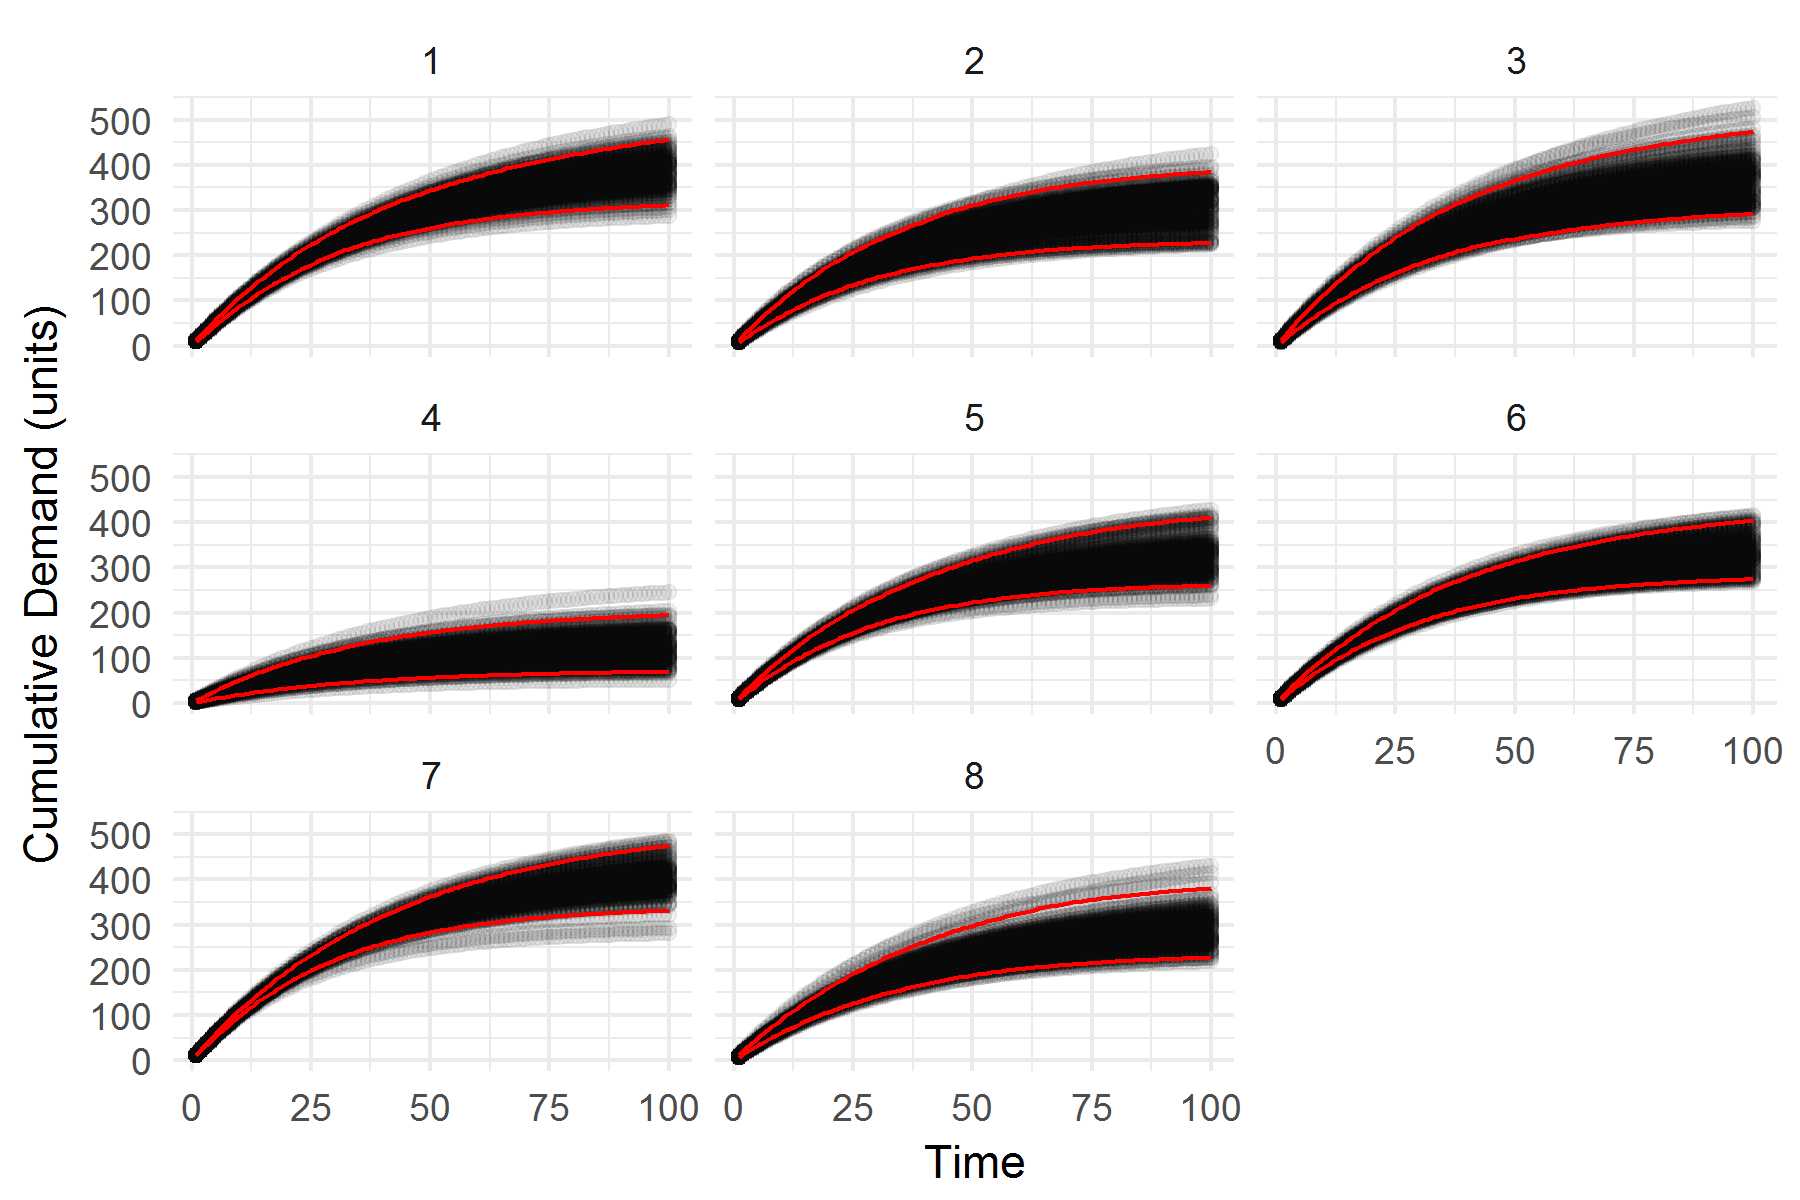
\includegraphics{demand-curve-95pct}
\caption{95\% credible intervals for cumulative demand curve in each region.}  \label{fi:demcurve}
\end{figure}

We determined an appropriate buy by deriving the posterior distribution of the cumulative demand across all regions at time $t = 100$.  The $90^{th}$ percentile of the posterior predictive distribution of demand was \SI{2828} units.  That number was selected as the buy, so $b = 2828$.

The most complicated part of the simulated example was the specification of the rules for fulfillment of orders.  The general strategy is to minimize $\sum_{k = 1}^K \sum_{i = 1}^{n_{kt}} c_1 (f_{tki}, h_{tki})$, the total cost of fulfillment, at any time point $t$.  At time points for which all fulfillment centers had sufficient remaining inventory to deliver to all of the ordering households for which it was the closest center, the fulfillment rule was simple --- households receive their order from the closest fulfillment center.  At time points for which fulfillment cannot be satisfied by the fulfillment center closest to a household placing an order, a sequential deterministic rule was used to reassign fulfillment to other centers.  Across all of the fulfillment centers with insufficient inventory to fulfill an order, we calculated the distance from the fulfillment centers with excess inventory to each of the ordering households.  The household with the minimum distance from a fulfillment center with excess inventory was moved from its currently assigned under-stocked fulfillment center to that alternate fulfillment center.  On days in which the total inventory across fulfillment centers was less than the total orders, a random set of orders was selected to fulfill.

We specified the cost functions associated with fulfillment and accelerating sales of excess inventory as follows:

$$c (f, h) = 5 + 5 d_1(f, h) + 2 d_2(f, h)$$

\noindent and

$$m (b, d^*) = 29.99 \exp \{- 0.00069 (b - d^*) \}.$$

\noindent where $d_1(\cdot, \cdot)$ is Euclidean distance and $d_2 (\cdot, \cdot)$ is a step function, $d_2 (f, h) = \lfloor 10 d_1(f, h) \rfloor$.  For concreteness, $d_1(\cdot, \cdot)$ can be thought of as the driving distance from the fulfillment center to the household and $d_2 (\cdot, \cdot)$ can be thought of as the number of days to deliver to the household from the fulfillment center.  The value of \SI{29.99} was selected arbitrarily as an AUR over the planned sales period.  The value of $\delta = 0.00069$ was selected so that an overstock of \SI{1000} units is associated with a markdown of approximately $50\%$ from AUR during the planned sales period.

One evaluation of $\mathbb{E}[\nu \mid \alpha_{10}, \alpha_{20}, \ldots, \alpha_{J0}]$ takes approximately 45 seconds on a single AWS processor.  The operation is easily parallelized, but for this proof-of-concept implementation we chose to reduce the set of initial inventory allocations explored and execute the process sequentially.  The set of initial allocations consisted of the $G = 125$ combinations of $\alpha_{10} = 100, 200, \dots, 500$; $\alpha_{20} = 300, 400, \dots, 700$; and $\alpha_{30} = 500, 800, \ldots 900$.  Each combination was assessed using $L = 100$ Monte Carlo simulations.

\subsection{Results}

Because the analysis was performed on a coarse grid, a statistical model was fitted to the observed estimates of expected value to obtain a final estimate of the optimal initial allocation.  Figure~\ref{fi:modelbroad} shows the estimated values of $\mathbb{E}[\nu]$ (points) and fitted model (lines) for selected levels of initial allocation to fulfillment center 1 (rows), fulfillment center 2 (columns), and fulfillment center 3 (x-axis).  In this figure, the y-axis shows the deviation from the optimal estimated point in dollars.  In this figure, the optimal allocation is obtained in the panel with $\alpha_{10} = 400$ (row) and $\alpha_{20} = 600$ (column), and the optimal fitted value is at $\alpha_{30} = 680$.  Using the fitted model to refine the estimate, the optimal point is identified as $\alpha_{10} = 418$, $\alpha_{20} = 571$, $\alpha_{30} = 682$, and $\alpha_{40} = 1157$.

\begin{figure}
\centering
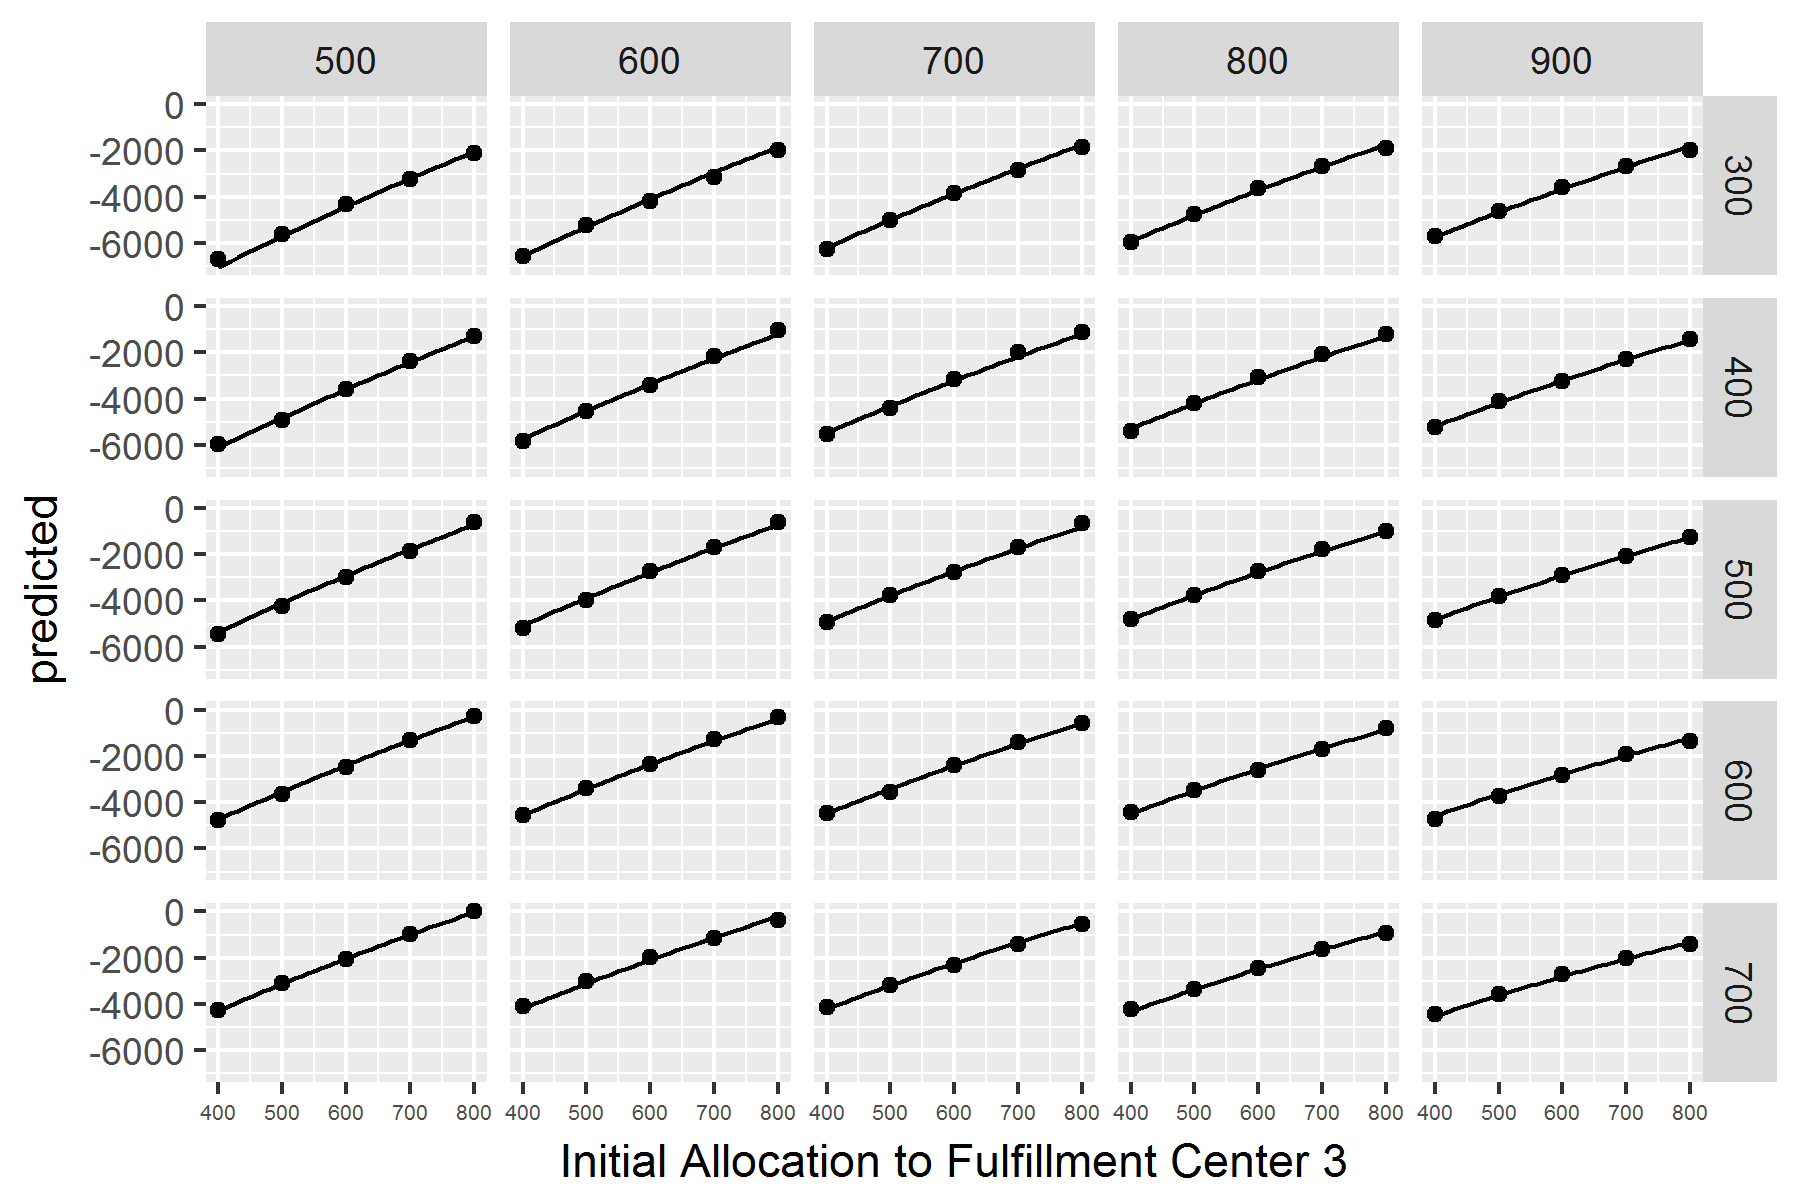
\includegraphics{model-fit-broad}
\caption{Estimated deviation from optimal value (points) and fitted model (lines) for selected levels of allocations to fulfillment centers.}  \label{fi:modelbroad}
\end{figure}


\end{document}  


